\section{Deployment Platform} \label{sec:system-architecture}
Our proposed deployment platform comprises five main components; pipeline manager, data manager, scheduler, proactive trainer, and the execution engine.
Figure \ref{fig:system-architecture} gives an overview of the architecture of our system and the interactions among its components.
At the center of the deployment platform is the pipeline manager.
The pipeline manager monitors the deployed pipeline and model, manages the processing of the training data and prediction queries, and enables the continuous update of the deployed model.
The data manager and the scheduler enable the pipeline manager to perform proactive training.
The proactive trainer component manages the execution of the iterations of SGD on the deployed model.
The execution engine is responsible for executing the actual data transformation and model training components of the pipeline.
The proposed design decouples the components of the platform from the execution engine.
This design enables us to switch the execution engine without requiring changes to the deployment platform.

\subsection{Scheduler}\label{scheduler}
The scheduler component is responsible for scheduling the proactive training.
The scheduler communicates with pipeline manager to instruct when to execute the proactive training.
The scheduler accommodates two types of scheduling mechanisms, namely \textit{static} and \textit{dynamic}.

The static scheduling utilizes a user-defined parameter that specifies the interval between executions of the proactive training.
This is a simple mechanism for use cases that require constant updates to the deployed model (for example, every minute).
The dynamic scheduling tunes the scheduling interval based on the rate of the incoming prediction, prediction latency, and the execution time of the proactive training.
The scheduler uses the following formula to compute the time when to execute the next proactive training:
\todo[inline]{Explain the parameters and the reason behind them in more detail}
\begin{center}
$T' = S * T * pr * pl$
\end{center}
where $T'$ indicates the time in seconds when the next proactive training is scheduled to execute, $T$ is the execution time of the last proactive training, $pl$ and $pr$ are the average prediction latency and the average number of prediction requests per second.
$S$ is the slack parameter.
Slack is a user-controlled parameter to hint the scheduler about the possibility of surges in the incoming prediction queries and training data.
A large slack value ($\geq10$) results in a larger scheduling interval, thus allocating most of the resources of the deployment platform to the query answering component.
A small slack value ($10 \geq S \geq 2$) results in smaller scheduling intervals.
As a result, the deployment platform allocates more computing resources for training the pipeline.
A slack value of less than 2 increases the latency of prediction answering component.

The scheduler computes the value of $T$ for every proactive training.
The deployment platform provides the scheduler with the values of $pr$ and $pl$. 
By utilizing the formula, the scheduler ensures that the platform has enough time to answer all the existing prediction queries before scheduling the next proactive training.
\begin{figure}[h]
\centering
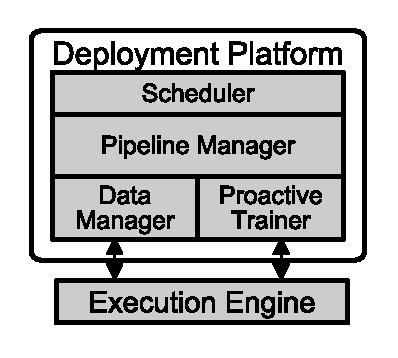
\includegraphics[width=\columnwidth]{../images/system-architecture.pdf}
\caption{System Architecture}
\label{fig:system-architecture}
\end{figure}


\subsection{Data Manager} \label{data-manager}
The data manager component is responsible for storage of historical data and cached features, receiving the incoming training data, and providing the proactive trainer with samples of the historical data.

Historical data is typically large and may not fit in the memory or disk of a single machine. 
The data manager handles the communication with the underlying storage unit.
The data manager has four tasks.
It appends the incoming training data to the historical dataset.
It forwards the incoming training data and prediction requests to the pipeline manager for further processing.
After the pipeline manager transforms the data into features, the data manager stores the transformed features.
Finally, upon the request of the pipeline manager, the data manager samples the historical data for proactive training.

If the feature materialization optimization is enabled, the data manager caches the transformed features.
During the sampling operation, instead of sampling from the raw historical data, the data manager samples from the transformed features directly.

The data manager provides three sampling approaches, namely, uniform, time-based, and window-based sampling.
Uniform sampling provides a random sample from the entire historical data where every data point has the same probability of being sampled.
Time-based sampling assigns weights to every data point based on their timestamp.
In time-based sampling, recent items have a higher probability of being sampled.
Window-based sampling is similar to the uniform sampling, however, instead of sampling from the entire historical data, the data manager samples the data from a given time range. 
In many real-world use cases (e.g., e-commerce and online advertising), the deployed model should adapt to the more recent data.
Therefore, the time-based and window-based sampling provide more appropriate samples for the training data.
However, in some use cases, the incoming training data is not time-dependent (e.g., image classification of objects).
In these scenarios, window-based sampling fails to provide a non-biased sample, since it only samples from the recent data.
In our experiments, we show that the time-based sampling satisfies the requirement of both types of use cases.

To increase the performance of the sampling operation, we utilize a data partitioning technique.
Upon the arrival of new training data, the data manager assembles a partition of the data and creates an index for the partition using the timestamps of the data that resides in the partition.
As a result, during the sampling operation, the data manager can access the data for a specific interval quickly.
To further speed up the sampling, the data manager randomly samples the partitions instead of individual data points.
The data manager combines the sampled partitions and sends the data to the pipeline manager.

The data manager also allows for new training datasets to be registered while the model is being served.
The new dataset is merged with the existing historical data and immediately becomes available for proactive training.

\subsection{Pipeline Manager} \label{pipeline-manager} 
The pipeline manager is the main component of the system.
It loads the pipeline and the trained model, transforms the data into features using the pipeline, enables the execution of the proactive training, and exposes the model to answer prediction queries.

During the online training, when new training data becomes available, the pipeline manager first transforms the data using the pipeline and updates the model.
During the online training, the pipeline manager also updates and stores the statistics of the pipeline components.
If the feature materialization optimization is enabled, the pipeline manager sends the transformed features to the data manager.

The scheduler component informs the pipeline to execute proactive training.
Then, the pipeline manager requests the data manager to provide the sample of the historical data for the next proactive training.
The pipeline manager provides the proactive trainer with the current model parameter and the sample of the historical data.
Once the proactive training is over, the pipeline manager receives the updated model.

The data manager also forwards prediction requests to the pipeline manager.
Similar to training data, the pipeline manager sends the prediction query through the pipeline to perform the necessary data preprocessing.
Using the same pipeline to process both the training data and prediction query guarantees that the same set of transformations are applied to both types of data.
As a result, the pipeline manager prevents inconsistencies between training and serving that is a common problem in machine learning model deployment \cite{baylor2017tfx}.
After preprocessing the prediction query, the pipeline manager uses the model to make a prediction.

\subsection{Proactive Trainer} 
The proactive trainer is responsible for training the deployed model by executing iterations of SGD.
In the training process, the proactive trainer receives a training dataset (sample of the historical data) and the current model parameters from the pipeline manager.
Then, the proactive trainer performs one iteration of SGD and returns the updated model to the pipeline manager.
The proactive trainer utilizes advanced learning rate adaptation techniques to dynamically adjust the learning rate parameter when training the model.
Although individual proactive training instances are independent of each other, the component must store the information required by the learning rate adaptation technique.
Lastly, the proactive trainer is the only component that is tightly coupled with the execution engine.
It directly executes the SGD logic on the execution engine.

\subsection{Execution Engine}
The execution engine is responsible for executing the SGD and prediction answering logic.
In our deployment platform, any data processing platform capable of processing data both in batch mode (for proactive training) and streaming mode (online learning and answering prediction queries) is a suitable execution engine.
\todo[inline]{Move the rest to the evaluation setup}
Apache Spark \cite{zaharia2010spark} is a distributed data processing platforms that can support both stream and batch data processing.
It works with data in memory and on disk which speeds up the execution of the proactive training.

In our current prototype, we are using Apache Spark as the execution engine.
The data manager component utilizes the Hadoop Distributed File System (HDFS) for storing the historical data \cite{shvachko2010hadoop}.
We leverage some of the components of the machine learning library in Spark to implement the proactive trainer.
Moreover, we utilize the caching mechanism of the Apache Spark for materializing the transformed features.
